\documentclass{article}
\usepackage{graphicx} % Required for inserting images
\usepackage{listings}
\usepackage{xcolor}
\lstset{
  language=Python,
  backgroundcolor=\color{gray!10}, % choose the background color; you must add \usepackage{color} or \usepackage{xcolor}
  basicstyle=\tiny\ttfamily, % the size of the fonts that are used for the code
  breaklines=false,                 % sets automatic line breaking
  breakatwhitespace=true,          % sets if automatic breaks should only happen at whitespace
  frame=single,                    % adds a frame around the code
  rulecolor=\color{black},         % if not set, the frame-color may be changed on line-breaks within not-black text (e.g. comments (green here))
  keywordstyle=\color{blue},       % keyword style
  commentstyle=\color{gray},       % comment style
  stringstyle=\color{orange},      % string literal style
  numbers=left,                    % where to put the line-numbers; possible values are (none, left, right)
  numberstyle=\tiny\color{gray},   % the style that is used for the line-numbers
  stepnumber=1,                    % the step between two line-numbers. If it's 1, each line will be numbered
  numbersep=10pt,                  % how far the line-numbers are from the code
  showspaces=false,                % show spaces everywhere adding particular underscores; it overrides 'showstringspaces'
  showstringspaces=false,          % underline spaces within strings only
  showtabs=false,                  % show tabs within strings adding particular underscores
  tabsize=2                        % sets default tabsize to 2 spaces
}

\title{Conjugate Gradient with Preconditioning}
\author{QuirkyCroissant, 2024}
\date{May 2024}

\begin{document}

\maketitle

\section*{Convergence behavior of Block Jacobi}

\textit{Compare the convergence behaviour for the different block sizes and matrices. Which block size performs better? For which matrix does the method work better? }

\begin{itemize}
    \item The Block Jacobi Method for Nos5 matrix performs almost similar in both block size executions(Blocksize 1 and 5). It starts at $10^{-1}$ but stays relatively the same.
    \item The Convergence of NOS6 on the other hand looks a little different. Both executions seem to converge, signified that both residuals drop significantly and even start at the low value of $10^{-7}$ for blocksize 1 and $9*10^{-8}$ for blocksize 5. So blocksize 5 performs better.
    \item In direct comparison NOS6 matrix performs better with our algorithm. indicated by the convergence indicated by the small and dropping residual.

\end{itemize}
 
    
\section*{Convergence of CG vs PCG}

\textit{Compare the convergence behaviour of unpreconditioned CG and of PCG with the different preconditioners for the two test matrices. Which preconditioner performs best for the respective matrix? What could be the reason for that? Do you see a relation to the respective results shown in Part 1? 
If yes, explain this relation. If no, explain what you would have expected from the results in Part 1.} 

\begin{figure}[h!]
    \centering
    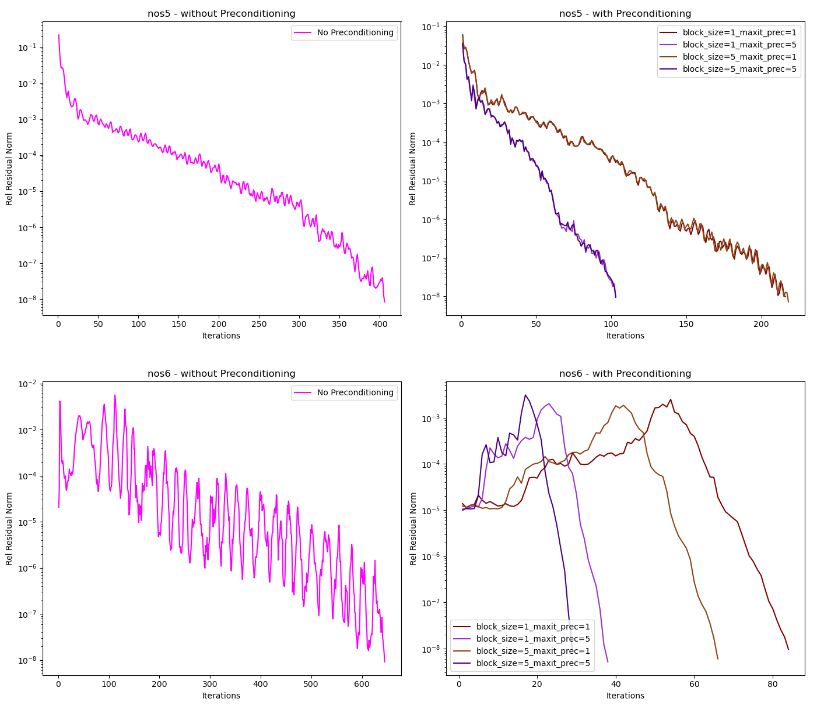
\includegraphics[width=1\linewidth]{pcg_vs_cg.PNG}
    \caption{Convergence CG vs PCG}
\end{figure}

\subsubsection*{unpreconditioned CG:}
\begin{itemize}
    \item Nos5 converges slowly with small oscillations in 400 iterations.
    \item Nos6 oscillates even more extreme and needs more than 600 iterations to converge.

\end{itemize}

\subsubsection*{preconditioned CG:}

\subsubsection*{Nos5} 

\begin{itemize}
    \item "blocksize1 and prec\_maxiterations 5" and "blocksize5 and prec\_maxiterations 5" converged the best with about 100 iterations.
    \item "blocksize1 and prec\_maxiterations 1" and "blocksize5 and prec\_maxiterations 1" performed not as good as the other two but are still a lot better than the unpreconditioned variante, both converge at about 220 iterations.

\end{itemize}


\subsubsection*{Nos6} 

Similarly to before "blocksize 5 and prec\_maxiterations 5" and "blocksize 1 and prec\_maxiterations 5" perform optimal with a convergence at about 30 and 38 iterations(really fast). Whereas "blocksize 5 and prec\_maxiterations 1" and "blocksize 1 and prec\_maxiterations 1" need about double the time of their previously mentioned counterparts with convergence seemingly kicking in at about 64 and 85 iterations.

Interesting observation is that all variants first diverge in their initial iterations before plummeting to a really good solution.

\subsection*{Potential Reasons and Reflexion to Part 1:}

First of all it seems that many iterations of preconditioning help both matrices in the speed of their overall convergence. With Matrix Nos6 explicitly it also seems to help to have bigger block sizes, because the executions with 5 as blocksize outperform their counterparts with only 1 as block size significantly. Seems that computational problems that the matrix has can be mitigated more with larger blocks.

We can also see some parallels to tast 1. where with matrix nos5 block size did not seem to help a lot in convergence, but with nos6 we can clearly see that a larger blocksize gives us the better residual.

\section*{Performance Table of CG vs PCG}

\begin{table}
\centering

\begin{tabular}{l l l}
Matrix Type & Execution Type & Runtime (sec) \\
nos5 & no-prec & 0.009997 \\
nos5 & block\_size=1, maxit\_prec=1 & 0.084496 \\
nos5 & block\_size=1, maxit\_prec=5 & 0.137000 \\
nos5 & block\_size=5, maxit\_prec=1 & 0.066000 \\
nos5 & block\_size=5, maxit\_prec=5 & 0.183002 \\
nos6 & no-prec & 0.029001 \\
nos6 & block\_size=1, maxit\_prec=1 & 0.074996 \\
nos6 & block\_size=1, maxit\_prec=5 & 0.084984 \\
nos6 & block\_size=5, maxit\_prec=1 & 0.031017 \\
nos6 & block\_size=5, maxit\_prec=5 & 0.050965 \\

\end{tabular}

\end{table}

 \begin{itemize}
    \item No preconditioned runs are by far the fastest, but we also saw from task 1 and 2 that they need longer to converge and we don't reach as good of a residual norm as with the conditioned variants.
    \item Nos5:
    \begin{itemize}
        \item Block\_size=1, maxit\_prec=5 and block\_size=5, maxit\_prec=5 perform the best in terms of convergence but they also need the longest to compute with 0.137 and 0.183 seconds.
        \item Block\_size=1, maxit\_prec=1 and block\_size=5, maxit\_prec=1 run the fastest but also perform less well as the runs with maxit\_prec=5.
    \end{itemize}
    \item Nos6:
    \begin{itemize}
        \item All executions run faster on average than with Nos5 matrix.
        \item Again block\_size=1, maxit\_prec=5 and block\_size=5, maxit\_prec=5 perform the best in terms of convergence, but they also lie at the lower end of runtime - with the former being the slowest of the variants with 0.085 seconds.
        \item Block\_size=5, maxit\_prec=1 performs better than block\_size=1, maxit\_prec=1 in terms of convergence, and in terms of speed it looks no different.
    \end{itemize}
\end{itemize}

For both matrix types we observe that a larger block size helps with convergence. Precondition the problem also helps with convergence but it comes at the cost that the algorithm now needs to run additional "iterations" to condition the matrix which costs more time of course.


\end{document}

